\section{GinVoice}\label{sec:ginvoice}
In dit hoofdstuk gaan we kijken naar GinVoice — een open-source Python GTK-applicatie die onder water \LaTeX\ gebruikt om facturen te maken.
Daarnaast nemen we de meegeleverde factuurtemplate onder de loep en kijken we naar de betrokken data binnen de factuur.

\subsection{De Applicatie} 

\looseness-1
De applicatie heeft meerdere weergaves.
De meest voorkomende weergave is de hoofdweergave, waarin je meerdere facturen tegelijkertijd kunt opstellen.
In deze weergave, te zien in figuur~\ref{fig:app}, zijn bijna alle onderdelen terug te zien.
Zo zie je de \textit{header}, \textit{informatietabellen}, \textit{factuurregels} en de \textit{slottekst} erin terug komen.
In figuur~\ref{fig:app} kun je zien dat de invoervelden al zijn ingevuld en dat de inhoud daarvan niet veel afwijkt als je het vergelijkt met het eindresultaat, te zien in figuur~\ref{fig:voorbeeldfactuur}.
Er komen later in dit hoofdstuk nog andere applicatie weergaves naar voren.


\subsection{\LaTeX-template}
Hieronder vind je een voorbeeld van de code binnen de \texttt{document} omgeving:

%\vspace*{-12pt}

\lstinputlisting[name=invoice-original,language={[LaTeX]TeX},firstnumber=52,linerange={52-81},numbers=left,xleftmargin=15pt,label={lst:main},caption={\texttt{invoice.tex}}]{ginvoice/invoice-original.tex}

\begin{figure}[!h]
    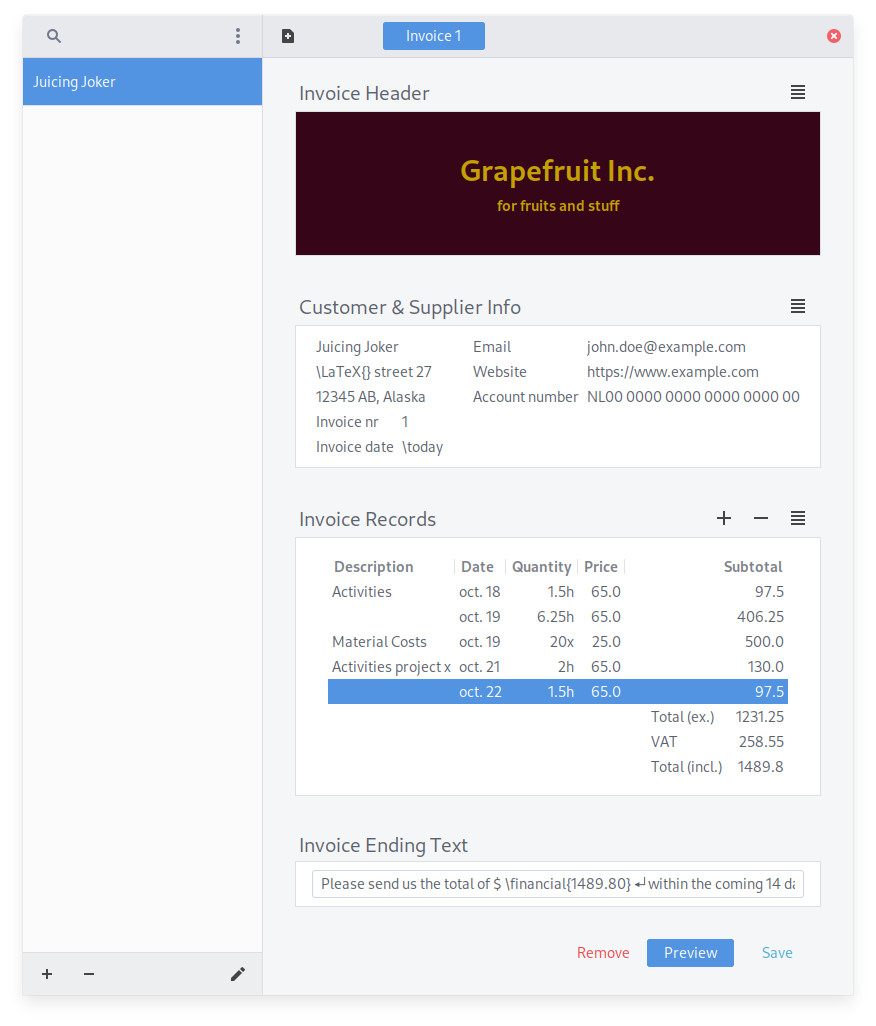
\includegraphics[width=\linewidth]{ginvoice/app.jpg}
    \caption{GinVoice — de applicatie}\label{fig:app}
\end{figure}


\begin{figure}[!h]
    \centering
    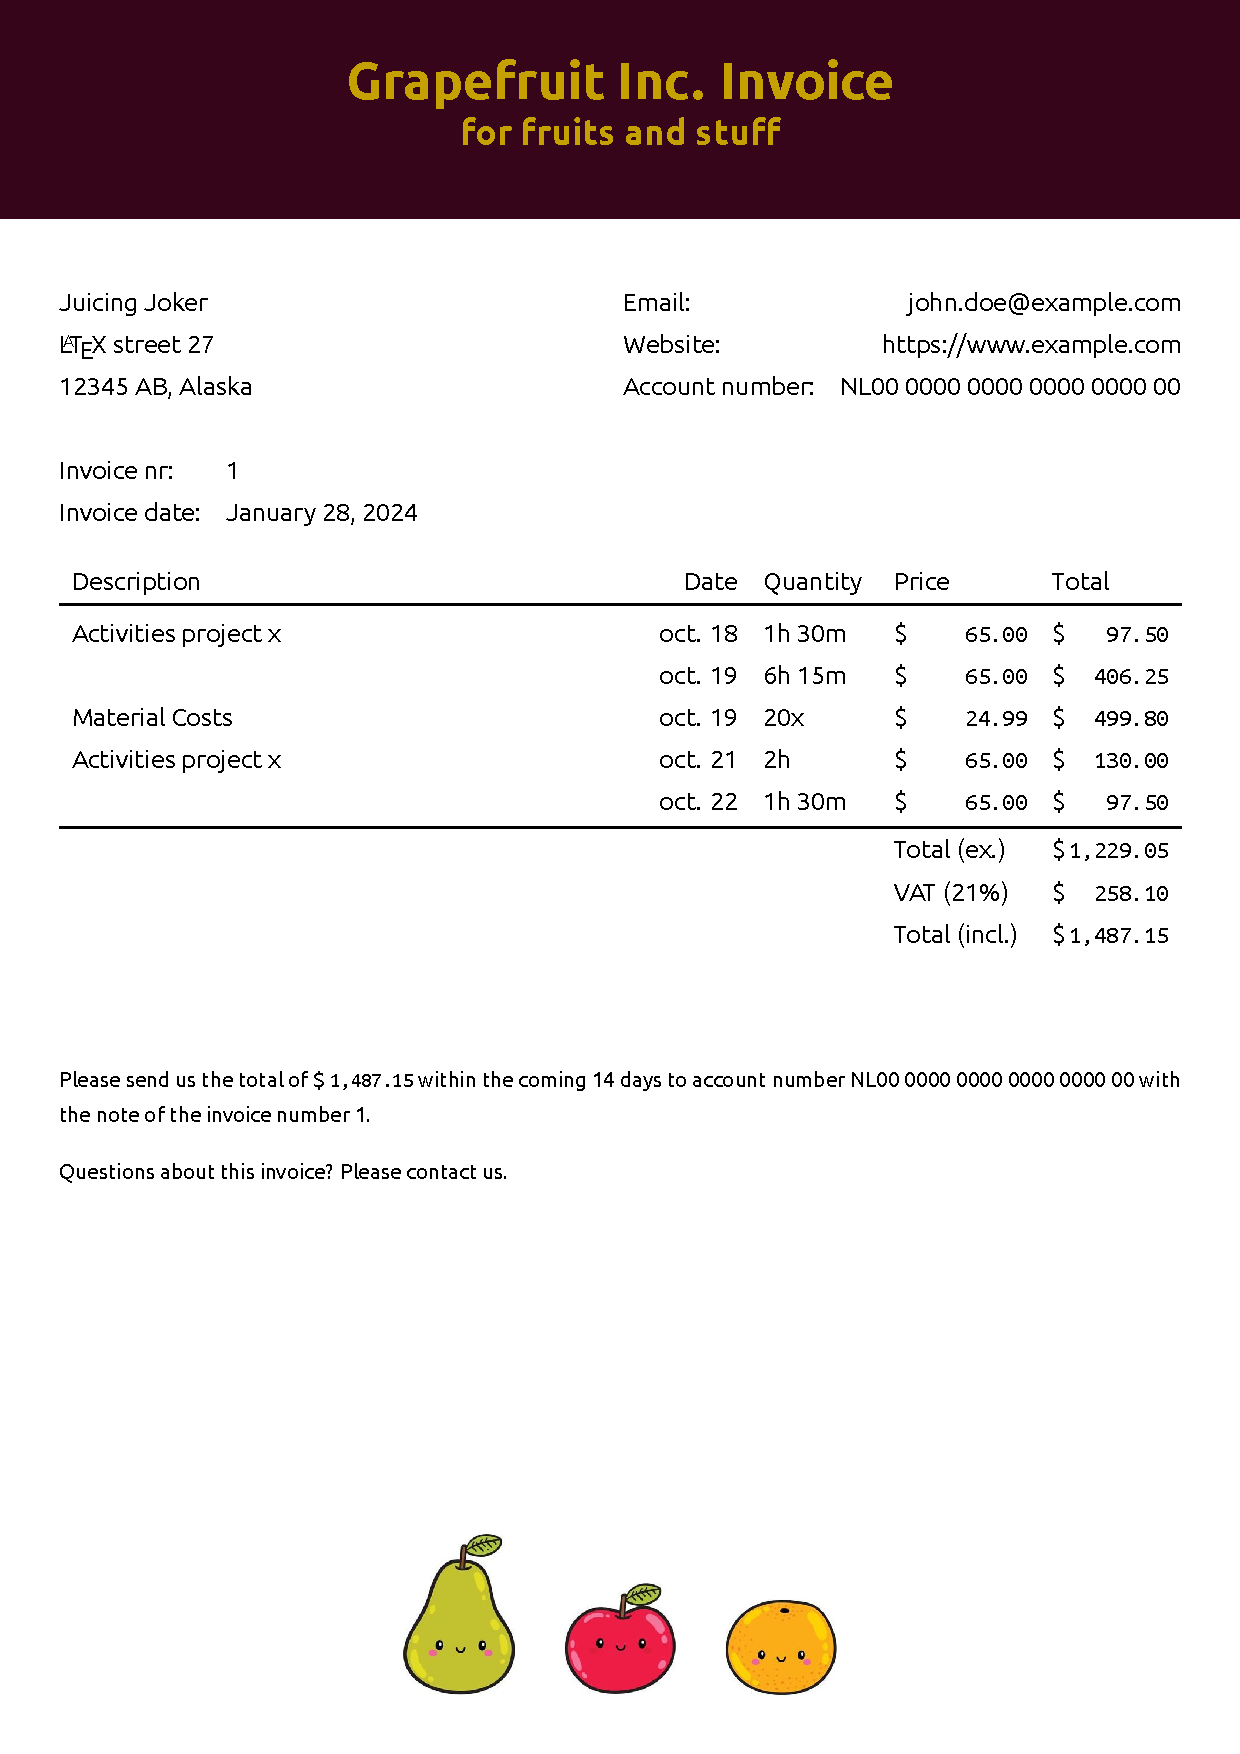
\includegraphics[width=.91\linewidth]{ginvoice/ginvoice.pdf}
    \caption{Voorbeeldfactuur gegenereerd met GinVoice\vadjust{\vspace*{-11pt}}}
    \label{fig:voorbeeldfactuur}
\end{figure}

De broncode in listing~\ref{lst:main} demonstreert verschillende macro's die vervangen zullen worden door \pkg{lua-placeholders}, waaronder \cs{title}, \cs{subtitle}, \cs{addressee}, \cs{customerinfo}, \cs{supplierinfo}, \cs{tablefooter}, \cs{tablerecords}, \cs{theending} en \cs{images}.
Daarnaast zijn er variabelen zoals stijl gerelateerde informatie en \cs{currency} die ook behandeld zullen worden.

\subsection{Gegenereerde \LaTeX-bestanden}
Het is belangrijk om te weten dat GinVoice\cite{ginvoice} momenteel een Python script -- \texttt{generator.py} -- gebruikt om extra \TeX-bestanden te genereren.
Deze \TeX-bestanden worden vervolgens in de template ingeladen met \cs{include}, zodat de benodigde macro's beschikbaar zijn.
%Echter, met de introductie van \pkg{lua-placeholders} zal deze aanpak niet langer nodig zijn.

Te beginnen met de taalinstelling:
\lstinputlisting[language={[LaTeX]TeX},caption={\texttt{languages.tex}}]{ginvoice/languages.tex}
Destijds heb ik ervoor gekozen om een aparte taalinstelling in de applicatie op te nemen te zien in figuur~\ref{fig:locale}, zodat woorden binnen de factuur netjes worden afgebroken met behulp van \pkg{babel}.

Een ander aspect binnen de preamble is het instellen van de documenteigenschappen.
Deze macro's komen mee vanuit het gegenereerde bestand \texttt{meta.tex}, waarvan de macro's later in het proces worden gebruikt in de \cs{hypersetup}.
\lstinputlisting[language={[LaTeX]TeX},caption={\texttt{meta.tex}}]{ginvoice/meta.tex}
Veelvoorkomende macro's, zoals \cs{title} worden op meerdere plekken gebruikt.
Dat is dan ook gelijk de reden waarom de \cs{title} niet in de \texttt{header.tex} hoeft te staan.
\lstinputlisting[language={[LaTeX]TeX},caption={\texttt{header.tex}}]{ginvoice/header.tex}
Het adres van de klant wordt in een macro gestopt, waarbij de adresregels van elkaar zijn gescheiden met behulp van een regeleinde.
\lstinputlisting[language={[LaTeX]TeX},caption={\texttt{addressee.tex}}]{ginvoice/addressee.tex}
Deze aanpak zou geschikt zijn voor een tabel met één kolom, of voor bijvoorbeeld een \texttt{enumerate} omgeving.

\begin{figure}[!t]
    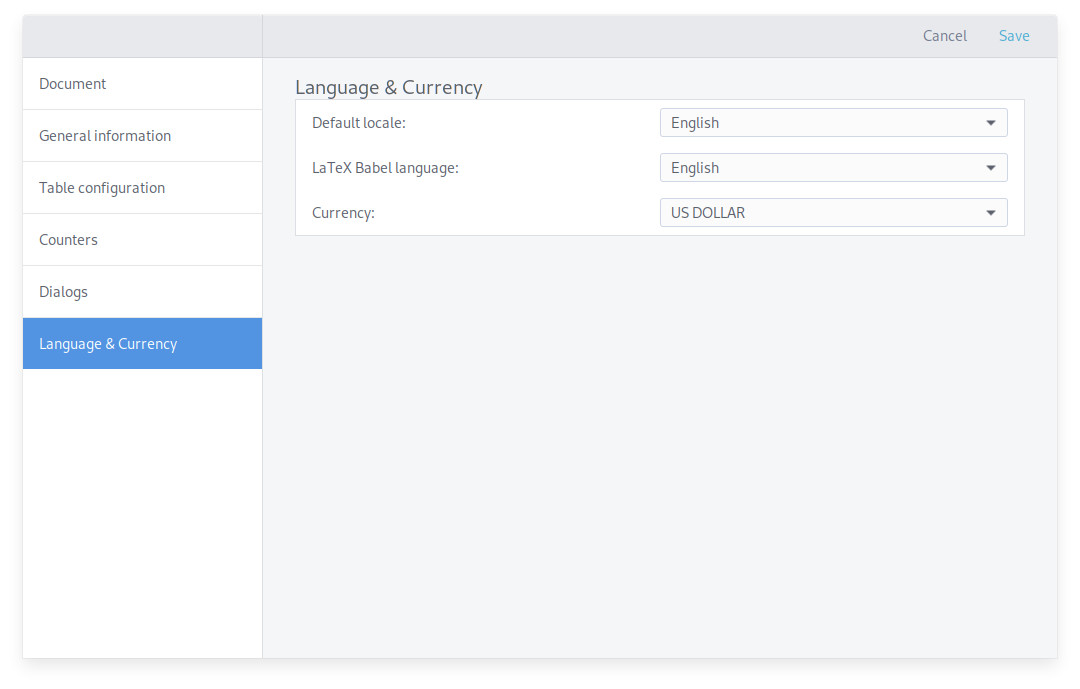
\includegraphics[width=\linewidth]{ginvoice/locale.jpg}
    \caption{Taalinstellingen}\label{fig:locale}
\end{figure}


De informatie van de klant en de leverancier gaat uit van een tabel omgeving met twee kolommen.

\vspace*{6pt}

\lstinputlisting[language={[LaTeX]TeX},caption={\texttt{customer\_info.tex}}]{ginvoice/customer_info.tex}
\lstinputlisting[language={[LaTeX]TeX},caption={\texttt{supplier\_info.tex}}]{ginvoice/supplier_info.tex}

\vspace*{12pt}

Het nadeel van deze opzet is dat een en-teken (\&) helemaal geen functie heeft binnen de context van de macro zelf.
Dat zou pas het geval zijn wanneer je binnen een \texttt{tabular} omgeving aan het werk bent.
Los van het feit dat de meeste \LaTeX-editors hierop een foutmelding geven, werkt deze aanpak gek genoeg alsnog.

De meest grote uitdaging binnen de applicatie was het configureerbaar maken van de factuurtabel.

Hiervoor is een aparte weergave, te zien in figuur~\ref{fig:tableconfig}.
In het figuur zie je dat iedere kolom een andere breedte kan hebben.
Dit kan zijn: de lengte van een stuk tekst, zo groot mogelijk, of verborgen.
Deze toegevoegde complexiteit vanuit de applicatie heeft destijds{\parfillskip0pt\par\newpage\aftergroup\noindent}een behoorlijk complexe uitkomst gehad op het gegenereerde \texttt{table.tex} bestand, te zien in de volgende code:
\lstinputlisting[language={[LaTeX]TeX},caption={\texttt{table.tex}}]{ginvoice/table.tex}

\newpage
Naast de complexe kolom configuratie heb je \cs{tablerecords} en \cs{tablefooter}, beide vergelijkbaar met bijvoorbeeld de \textit{leveranciersinformatie}.

\begin{figure}[!t]
    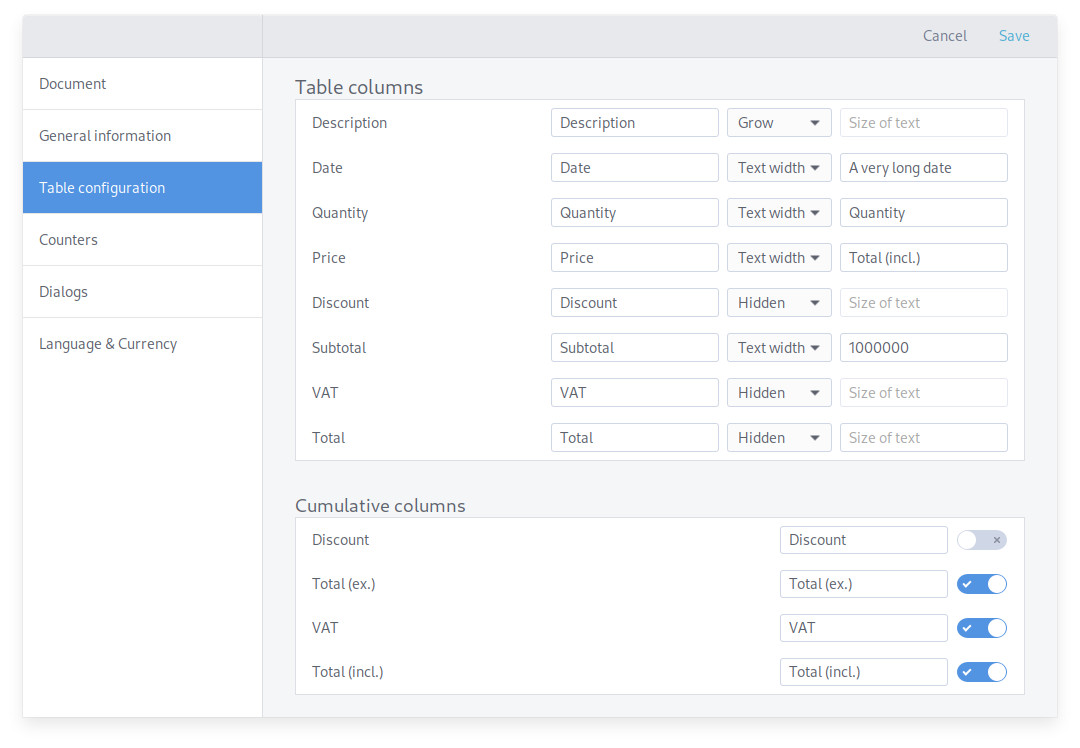
\includegraphics[width=\linewidth]{ginvoice/table-settings.jpg}
    \caption{Tabelinstellingen}\label{fig:tableconfig}
\end{figure}


Het laatste gegenereerde bestand \texttt{footer.tex} definieert de laatst ontbrekende macro's, \cs{theending} en \cs{images}:
\lstinputlisting[language={[LaTeX]TeX},caption={\texttt{footer.tex}}]{ginvoice/footer.tex}
Destijds heb ik er voor gekozen om alle grafische bestanden ergens binnen de omgeving van GinVoice op te slaan.
Dit heb weten te koppelen met \LaTeX\ door gebruik te maken van \cs{graphicspath}.

\newpage

\subsection{Factuurdata}\label{sec:invoice data}
Als we kijken naar alle informatie afkomstig uit GinVoice, met uitzonderingen daar gelaten, dan komen we uit op de data gepresenteerd in figuur~\ref{fig:klassendiagram}.

\begin{figure}[!t]
    \centering
    \begin{tikzpicture}
    \begin{class}[text width=5cm]{Invoice}{1.75,0}
        \attribute{title : String = Invoice}
        \attribute{subtitle : String}
        \attribute{currency : String = \cs{EUR}}
        \attribute{number : Number}
        \attribute{date : String = \cs{today}}
        \attribute{records : Table}
        \attribute{totals : Table/Object}
        \attribute{ending : String}
    \end{class}
    \begin{class}[text width=3cm]{Supplier}{3.5,-4.75}
        \attribute{email : String}
        \attribute{website : String}
        \attribute{accountnr : String}
    \end{class}
    \begin{class}[text width=3cm]{Client}{0,-4.75}
        \attribute{name : String}
        \attribute{street : String}
        \attribute{postal : String}
        \attribute{place : String}
    \end{class}
    \begin{class}[text width=4cm]{Style}{3,-7.5}
        \attribute{images : List}
        \attribute{main font : String}
        \attribute{mono font : String}
        \attribute{foreground color : String}
        \attribute{background color : String}
        \attribute{\sout{colored table} : Boolean}
    \end{class}
    \draw[umlcd style, diamond-angle 45] ($(Invoice.south west) - (-1.25,0)$) -- ($(Client.north) + (.375,0)$);
    \draw[umlcd style, diamond-angle 45] ($(Invoice.south east) + (-1.25,0)$) -- ($(Supplier.north) + (-.375,0)$);
    \draw[umlcd style, diamond-angle 45] ($(Supplier.south) + (-.375,0)$) -- ($(Style.north) + (.125,0)$);
\end{tikzpicture}

    \caption{Klassendiagram van de factuur}
    \label{fig:klassendiagram}
\end{figure}

Ik heb voor het gemak alvast alle informatie opgeknipt in aparte entiteiten, die overeen zullen komen met de YAML-bestanden, uitvoerig besproken in hoofdstuk~\ref{sec:new situation}.

%\subsection{Resultaat Voorbeeld}
%Het voorbeeld in figuur~\ref{fig:voorbeeldfactuur} toont een gegenereerde factuur met behulp van de huidige implementatie van GinVoice.
%\begin{figure}[!ht]
%    \centering
%    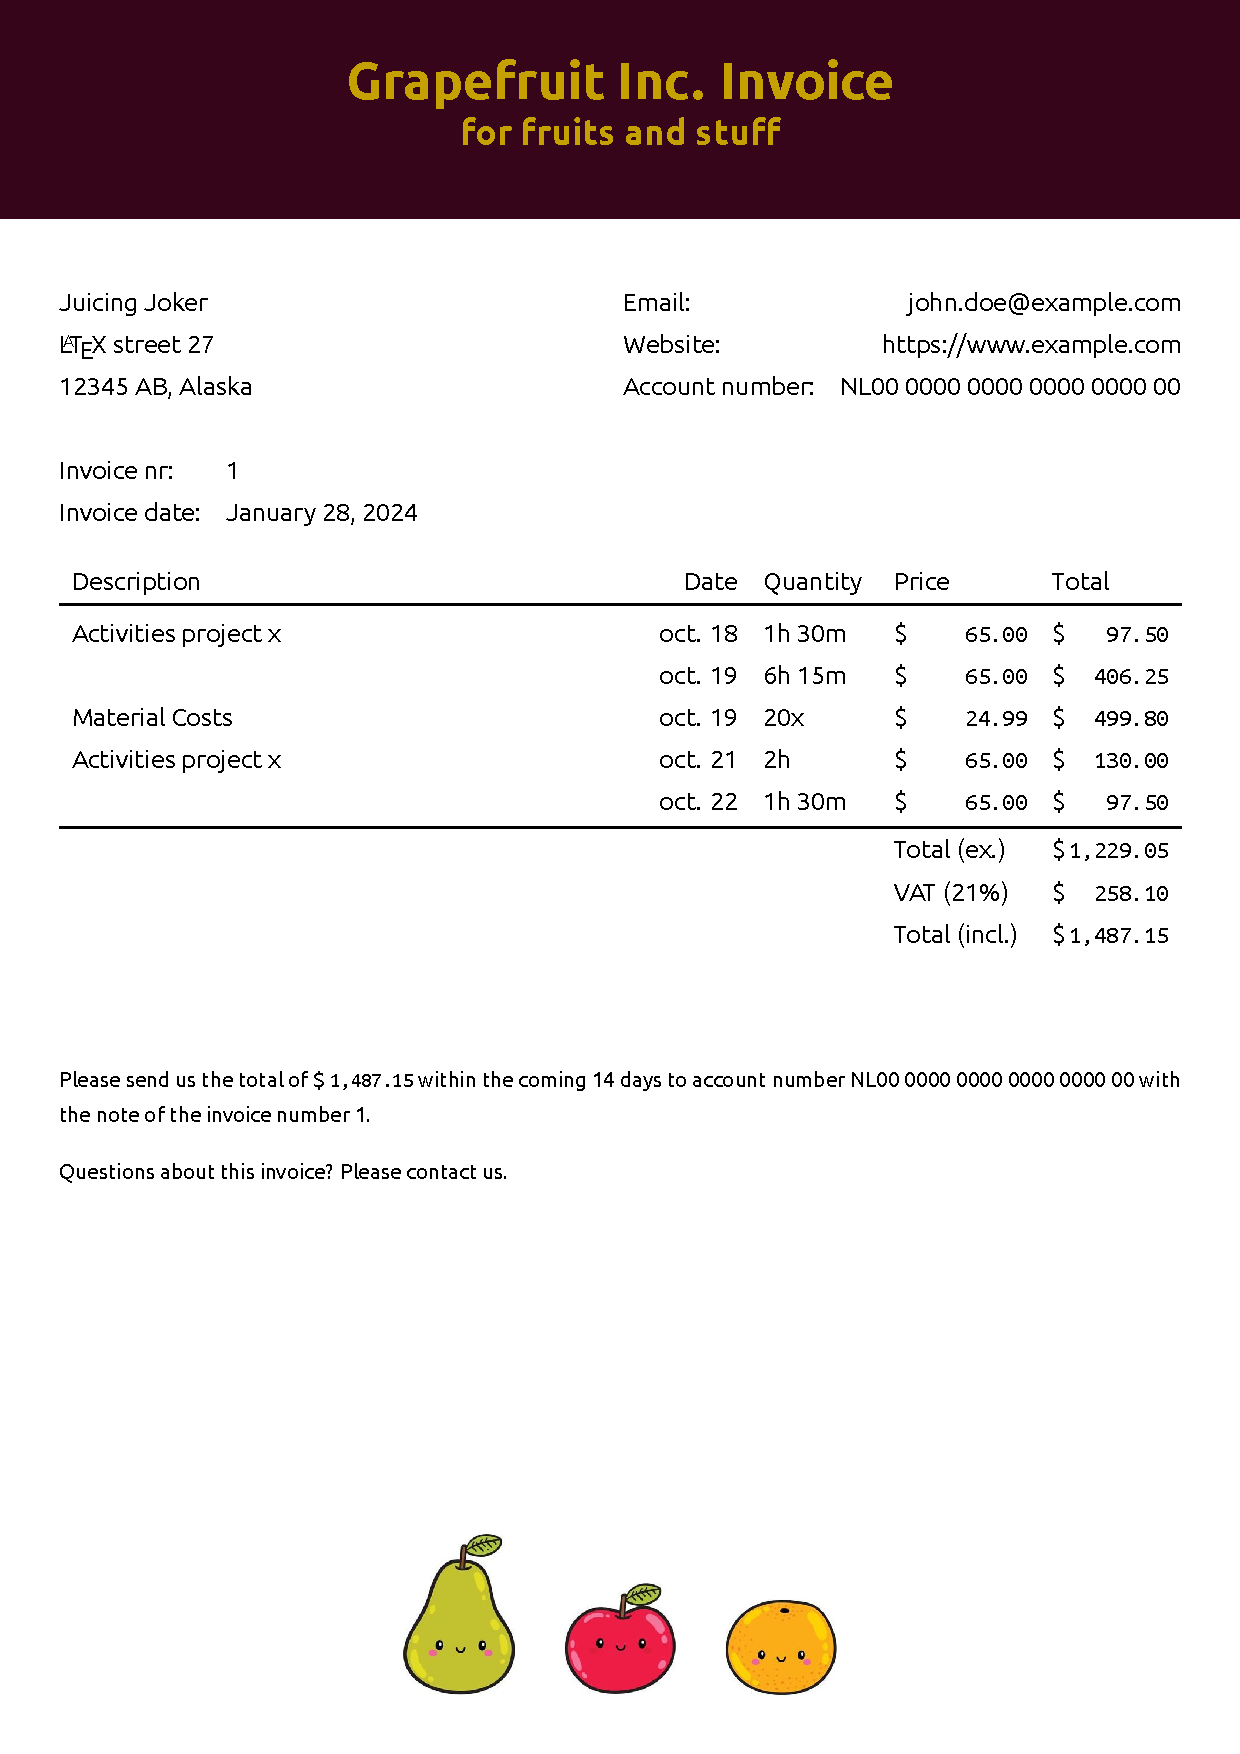
\includegraphics[width=\linewidth]{ginvoice/ginvoice.pdf}
%    \caption{Voorbeeldfactuur gegenereerd met GinVoice}
%    \label{fig:voorbeeldfactuur}
%\end{figure}
%Echter, op dit moment vereist het genereren van dit voorbeeld Python, wat voor template makers die hoofdzakelijk \LaTeX\ gebruiken, ongewenst is.
%In het volgende hoofdstuk zullen we deze situatie aanpakken en laten zien hoe dit voorbeeld rechtstreeks kan worden gegenereerd met \LuaLaTeX.
